\documentclass[a4paper,oneside,DIV=12,12pt,headings=normal]{scrartcl}

%%% Support for color
\usepackage{xcolor}
\definecolor{lightblue}{HTML}{03A9F4}
\definecolor{red}{HTML}{F44336}
%%%

%%% Links and hyperreferences
\usepackage{hyperref}
\hypersetup{
	colorlinks      = false,
	linkbordercolor = red,
	urlbordercolor  = lightblue,
	pdfborderstyle  = {/S/U/W 1.5},
}
%%%

%%% Graphics inclusion
\usepackage{graphicx}
%%%

%%% Font selection
\usepackage{fontspec}

\setromanfont{STIX Two Text}[
]

\setsansfont{Source Sans Pro}[
]

\setmonofont{Source Code Pro}[
	% Scale = 1.05,
]

% Used for suppressing polyglossia errors regarding missing cyrillic script
% \newfontfamily\cyrillicfonttt[
	% Script = Cyrillic,
	% Scale  = MatchUppercase,
% ]{Inconsolata}

\usepackage{unicode-math}
\setmathfont{STIX Two Math}

%%%

%%% Font settings for different KOMA Script elements
\setkomafont{pagenumber}{\rmfamily}
\setkomafont{disposition}{\rmfamily\bfseries}
%%%

%%% Typographic enhancements
\usepackage{microtype}
%%%

%%% Language-specific settings
\usepackage{polyglossia}
\setmainlanguage{ukrainian}
%%%

%%% List settings
\usepackage{enumitem}
\setlist[enumerate]{
	leftmargin = *,
}
%%%

%%% Captions
\usepackage{caption}
%%%

%%% Code listings
\usepackage{minted}

%%%

%%% Framing code listings
\usepackage{tcolorbox}
\tcbuselibrary{breakable}
\tcbuselibrary{minted}
\tcbuselibrary{skins}

\newtcbinputlisting[auto counter, list inside, number within = section]{\inputasm}[4][]{%
	minted language = nasm,
	minted style    = bw,
	minted options  = {
		linenos,
		tabsize = 4,
		breakbytokenanywhere,
		fontsize = \small,
	},
	%
	% empty,
	sharp corners,
	colframe         = black,
	colback          = black!0,
	leftrule         = 0em,
	rightrule        = 0em,
	toprule          = 0pt,
	bottomrule       = 0pt,
	titlerule        = 0.5pt,
	colbacktitle     = black!0,
	coltitle         = black,
	toptitle         = 0.3em,
	bottomtitle      = 0.1em,
	borderline north = {1pt}{0pt}{black},
	borderline south = {1pt}{0pt}{black},
	before skip      = \intextsep,
	after  skip      = \intextsep,
	title            = {Лістинг \thetcbcounter: #3},
	list entry       = {\protect\numberline{\thetcbcounter}#3},
	left = 0em,
	right = 0em,
	%
	listing file={#2},
	listing only,
	breakable,
	%
	label = {#4},
	%
	#1
}

% Customize minted line numbers
\renewcommand{\theFancyVerbLine}{\ttfamily\scriptsize\arabic{FancyVerbLine}}

%%%


\begin{document}
	\begin{titlepage}
	\centering
		Міністерство освіти і науки України\\
		Національний авіаційний університет\\
		Навчально-науковий інститут комп'ютерних інформаційних технологій\\
		Кафедра комп'ютеризованих систем управління

		\vspace*{\fill}

		Лабораторна робота №1\\
		з дисципліни «Системне програмування»\\
		на тему «Введення та виведення тексту»\\
		Варіант №4

		\vspace*{\fill}
		
		\begin{flushright}
			Виконав:\\
			студент ННІКІТ СП-225\\
			Клокун Владислав\\
			Перевірив:\\
			Сабрук І.~М.
		\end{flushright}

		Київ 2018
    \end{titlepage}
	
	\section{Мета роботи}
		Ознайомитись з синтаксисом та структурою програми на мові асемблера. Навчитися використовувати функції операційної системи для введення та виведення тексту. Дослідити різницю між файлами .COM та~.EXE.
		
	\section{Хід роботи}
		% Основним завданням роботи є розробка програми, до задач якої входять:
		% \begin{enumerate}
			% \item Введення рядка з клавіатури.
			% \item Вивід тексту на екран.
		% \end{enumerate}
		% В результаті виконання роботи була розроблена програма (ліст.~\ref{lst:01}).
				
		% \inputasm{../01-solution/01.asm}{Основна програма}{lst:01}
				
		% Додатковим завданням роботи було написання програми, яка виведе з введеного рядку на екран тільки парні за порядком літери. В результаті виконання роботи була розроблена відповідна програма (ліст.~\ref{lst:02}).
		Завданням роботи було написання програми, яка виведе з введеного рядку на екран тільки парні за порядком літери. В результаті виконання роботи була розроблена відповідна програма (ліст.~\ref{lst:02}).
				
		\inputasm{../01-solution/02.asm}{Додаткова програма}{lst:02}
		
		Після створення виконуваного файлу та роботи з програмою отримали необхідний результат (рис.~\ref{fig:02-run}).
		
		\begin{figure}[!htbp]
		\centering
			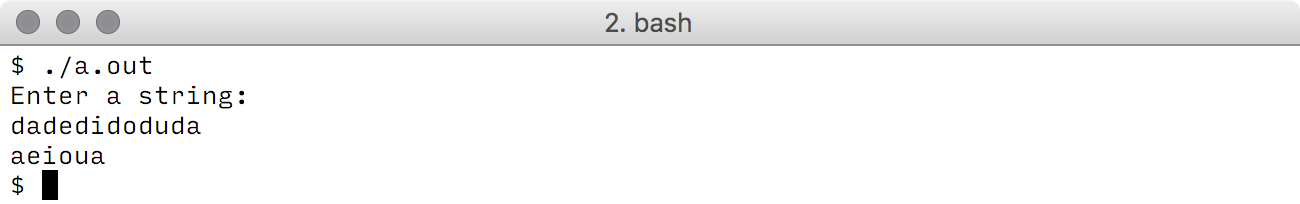
\includegraphics[width = \textwidth]{./assets/asmres.png}
		\caption{Результат роботи програми}
		\label{fig:02-run}
		\end{figure}
		
	\section{Висновок}
		Під час виконання даної лабораторної роботи ми ознайомились з синтаксисом та структурою програми на мові асемблера; навчились використовувати функції операційної системи для введення та виведення тексту, а також дослідили різницю між файлами .COM та .EXE.
\end{document}